\chapter{Motor-Driver Break-out Board DRV8833}

\begin{figure}[h]
	\centering
    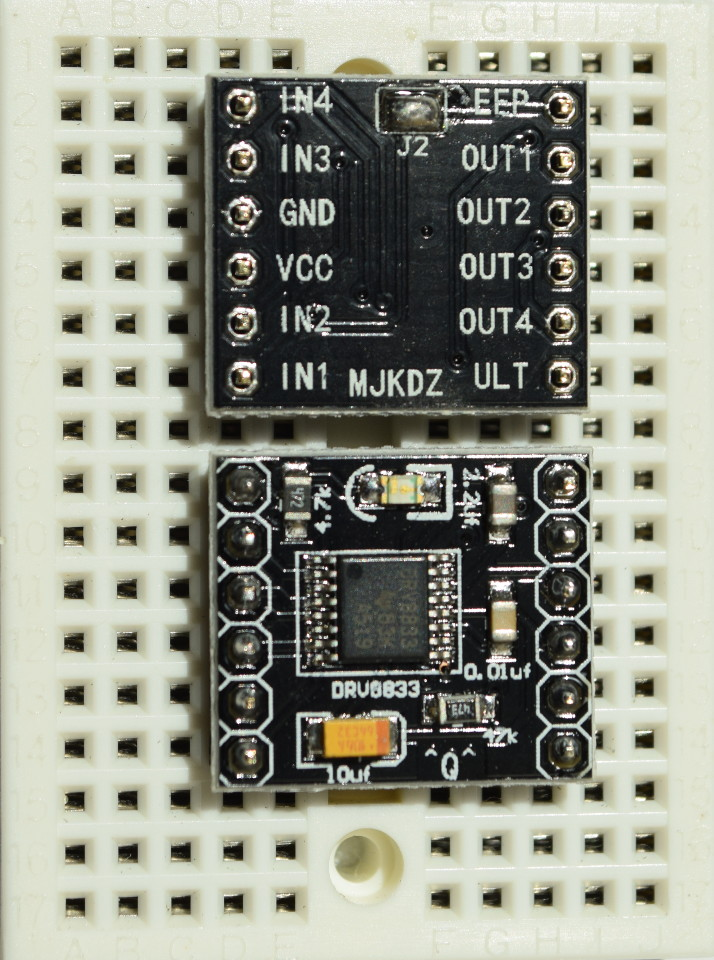
\includegraphics[width=0.5\textwidth]{photos/drv8833_breakout.jpg}
	\centering\bfseries
	\caption{DRV8833 Break-out board (2 boards showing with view of top and bottom sides)}
\end{figure}


The recommended motor driver IC is the Texas Instruments DRV8833:

\url{http://www.ti.com/lit/ds/symlink/drv8833.pdf}

This devices works perfectly with this project and is inexpensive.
Several eBay sellers offer a ``break-out board'' with the IC and several external components mounted with break-board friendly header pin holes.  The board shown in the photo above even includes a surface mounted LED power indicator!

The connections to the board are as follows:

\begin{enumerate}
\item ULT PIN:mode set. Low level is sleep mode
\item OUT1,OUT2:1-channel H-bridge controlled by IN1/IN2
\item OUT3,OUT4:2-channel H-bridge controlled by IN3/IN4
\item EEP PIN:Output protection. Default no need to connect.
\item VCC:3-10V
\item GND
\end{enumerate}

From the above list, only 2, 5 and 6 are used in this project.

IN1 is connected to the PWM output of the BBG, which is header P9.42.
The GND pin requires a connection to one of the grounds on the BBG such as P8.1 or P8.2.

VCC should be connected to an 8Volt DC power supply, however, the exact voltage is not critical.  A solid ground connection should be made between the 8Volt supply and the DRV8833 board.

OUT1 and OUT2 should be connected to the motor power terminals.

